\documentclass[aspectratio=169,11pt]{beamer}
\usetheme{Madrid}
\usecolortheme{default}
\usefonttheme{professionalfonts}

\usepackage[T1]{fontenc}
\usepackage[utf8]{inputenc}
\usepackage{lmodern}
\usepackage{amsmath,amssymb,mathtools}
\usepackage{booktabs}
\usepackage{tabularx}
\usepackage{array}
\usepackage{tikz}
\usetikzlibrary{arrows.meta,positioning,fit,calc}

\setbeamertemplate{navigation symbols}{}
\setbeamertemplate{footline}{\hfill\usebeamerfont{page number in head/foot}\insertframenumber\kern1em\vskip2pt}

\newcommand{\kk}{\Bbbk}
\newcommand{\R}{\mathbb{R}}
\newcommand{\Z}{\mathbb{Z}}
\newcommand{\Q}{\mathbb{Q}}

\title{Implementation of a Toolkit for Algebraic Module Encodings over $\R^n$ and Other Posets}
\subtitle{TAMER-OP}
\author{Erik Mendes Novak}
\date{April 7th 2026}

\begin{document}

\begin{frame}
  \titlepage
\end{frame}

% =========================================================
% Background slides to insert near the start of the deck
% =========================================================

\begin{frame}{Posets and persistence modules}
	\small
	A \emph{poset} is a set $Q$ with a relation $\leq$ that is reflexive,
	antisymmetric, and transitive.
	
	\vspace{0.5em}
	The main ambient posets in this talk are:
	\[
	\mathbb{Z}^n,\qquad \mathbb{R}^n,
	\]
	equipped with the coordinatewise order
	\[
	a \leq b \iff a_i \leq b_i \text{ for all } i.
	\]
	
	\vspace{0.5em}
	A \emph{persistence module over $Q$} is a functor
	\[
	M : Q \to \mathbf{Vect}_{\kk}.
	\]
	Equivalently:
	\begin{itemize}
		\item each $q \in Q$ carries a vector space $M(q)$,
		\item each relation $q \leq q'$ carries a linear map
		\[
		M(q \leq q') : M(q) \to M(q'),
		\]
		\item and these maps compose functorially.
	\end{itemize}
	
\end{frame}

\begin{frame}{Upsets, downsets, and indicator modules}
	\small
	Let $Q$ be a poset.
	
	\begin{block}{Order-theoretic regions}
		An \emph{upset} $U \subseteq Q$ satisfies
		\[
		q \in U,\ q \leq q' \Longrightarrow q' \in U.
		\]
		A \emph{downset} $D \subseteq Q$ satisfies
		\[
		q' \in D,\ q \leq q' \Longrightarrow q \in D.
		\]
	\end{block}
	
	\begin{block}{Indicator modules}
		To an upset $U$ we associate the module $\kk\{U\}$:
		\[
		\kk\{U\}(q)=
		\begin{cases}
			\kk, & q \in U,\\
			0, & q \notin U,
		\end{cases}
		\]
		with the obvious structure maps. Dually, a downset $D$ gives $\kk\{D\}$.
	\end{block}
\end{frame}
	
\begin{frame}{Upsts, downsets, and indicator modules}
	\vspace{0.4em}
	These indicator modules are the building blocks of presentations:
	\begin{itemize}
		\item upset indicators act like generators,
		\item downset indicators act like relations or cogenerators.
	\end{itemize}
	
	\vspace{0.4em}
	They are the persistence-module analog of the standard pieces used to
	present modules in commutative algebra.
\end{frame}

\begin{frame}{Fringe presentations}
	\small
	A \emph{fringe presentation} is a map
	\[
	\varphi :
	\bigoplus_{i=1}^{m} \kk\{U_i\}
	\longrightarrow
	\bigoplus_{j=1}^{r} \kk\{D_j\},
	\]
	where the $U_i$ are upsets and the $D_j$ are downsets.
	
	\vspace{0.5em}
	The module of interest is the image
	\[
	M = \operatorname{im}(\varphi).
	\]
	
	\vspace{0.5em}
	After choosing bases on the indicator summands, $\varphi$ is represented by
	a matrix
	\[
	\Phi \in \kk^{r\times m}.
	\]
	
	\vspace{0.5em}
	At a parameter value $q$, only some upsets and some downsets are active:
	\[
	I(q)=\{i : q \in U_i\}, \qquad J(q)=\{j : q \in D_j\}.
	\]
	The fiber $M(q)$ is then computed from the submatrix
	\[
	\Phi_{J(q),\,I(q)}.
	\]
\end{frame}

\begin{frame}{Fringe presentations}
	\vspace{0.5em}
	So a fringe presentation packages a module by saying:
	\begin{quote}
		which generators are present where, which relations are present where,
		and how they are linearly coupled.
	\end{quote}
\end{frame}

\begin{frame}{Three presentation types used before encoding}
	\small
	\renewcommand{\arraystretch}{1.25}
	\begin{tabular}{p{0.18\textwidth} p{0.22\textwidth} p{0.22\textwidth} p{0.28\textwidth}}
		\hline
		\textbf{Type} & \textbf{Ambient poset} & \textbf{Basic regions} & \textbf{Why it matters} \\
		\hline
		\textbf{Flange} &
		$\mathbb{Z}^n$ &
		flats and injectives &
		discrete input, adapted to finitely determined modules over $\mathbb{Z}^n$ \\
		
		\textbf{PL box} &
		$\mathbb{R}^n$ &
		axis-aligned upsets/downsets cut by coordinate thresholds &
		fastest real-parameter backend; threshold grid gives efficient traversal \\
		
		\textbf{PL fringe} &
		$\mathbb{R}^n$ &
		general piecewise-linear upsets/downsets given by polyhedra &
		more general geometry; needed when boundaries are not axis-aligned \\
		\hline
	\end{tabular}
	
	\vspace{0.2em}
	All three are mathematically the same kind of object:
	\begin{itemize}
		\item a presentation by indicator modules,
		\item but adapted to different ambient parameter spaces and geometries.
	\end{itemize}
	
	\vspace{0.2em}
	The encoding step converts all of them into the same output type:
	a finite poset $P$, an encoded module on $P$, and a classifier map
	\[
	\pi : \text{ambient space} \to P.
	\]
\end{frame}

\begin{frame}{Raw data as a fourth input type}
	\small
	Not every user begins with a presentation. Often the input is raw data:
	\[
	\text{point cloud},\ \text{graph},\ \text{image},\ \text{graded complex},\ \text{simplex tree}.
	\]
	
	\vspace{0.5em}
	A filtration specification turns that raw object into a finite graded object:
	\begin{itemize}
		\item simplicial or cubical complexes,
		\item graded chain or cochain complexes,
		\item and then modules or cohomology modules on a finite grid.
	\end{itemize}
	
	\vspace{0.5em}
	So there are really \textbf{four} front ends:
	\begin{enumerate}
		\item flange,
		\item PL box presentation,
		\item general PL fringe presentation,
		\item raw filtered data.
	\end{enumerate}
	
	\vspace{0.5em}
	The key design choice of the software is that these four very different inputs
	all flow into the same encoding-centered internal language.
\end{frame}

\begin{frame}{Tameness and finite encoding}
	\small
	\begin{block}{Finite encoding}
		A module $M$ over a large poset $Q$ is \emph{finitely encoded} if there exist
		\begin{itemize}
			\item a finite poset $P$,
			\item a monotone classifier map $\pi : Q \to P$,
			\item and a $P$-module $H$,
		\end{itemize}
		such that
		\[
		M \cong \pi^* H.
		\]
	\end{block}
	
	\begin{block}{Tame module}
		A module is \emph{tame} if it admits such a finite encoding.
	\end{block}
\end{frame}

\begin{frame}{Why is tameness good?}	

	\begin{itemize}
		\item It replaces an infinite or geometrically complicated parameter space by a finite one.
		\item It does \emph{not} throw away the module: the original module is recovered by pullback.
		\item It makes exact algebra possible: kernels, cokernels, Hom, Ext, Tor, mapping cones, and more can all be computed on the finite encoded object.
	\end{itemize}
	
	\vspace{0.5em}
	So the encoder is not producing a summary invariant. It is producing a
	finite, computable model of the module itself.
\end{frame}

\begin{frame}{The computational question}
\small
We want to replace a module on a large indexing poset by finite data
\[
M \cong \pi^* H,
\qquad
\pi:Q\to P,
\]
where $P$ is finite and $H$ is a module on that finite poset.

\medskip
\begin{itemize}
  \item the front end may live on $\Z^n$, $\R^n$, a finite poset, or come from filtered data;
  \item the output must be reusable for algebra, invariants, serialization, and visualization;
  \item this is why the workflow returns a full encoded object, not just a summary.
\end{itemize}

\medskip
\centering
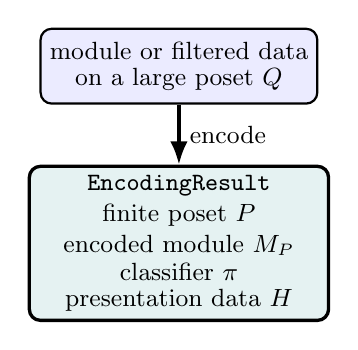
\begin{tikzpicture}[
  >=Latex,
  every node/.style={font=\small},
  box/.style={rounded corners, draw, thick, align=center, minimum width=3.1cm, minimum height=0.95cm, fill=blue!8},
  outbox/.style={rounded corners, draw, very thick, align=center, minimum width=3.8cm, minimum height=1.55cm, fill=teal!10}
]
\node[box] (in) at (0,1.45) {\shortstack{module or filtered data\\on a large poset $Q$}};
\node[outbox] (out) at (0,-0.8) {\shortstack{\texttt{EncodingResult}\\finite poset $P$\\encoded module $M_P$\\classifier $\pi$\\presentation data $H$}};
\draw[->,very thick] (in) -- node[right]{encode} (out);
\end{tikzpicture}
\end{frame}

\begin{frame}{Four front end input types}
\small
\centering
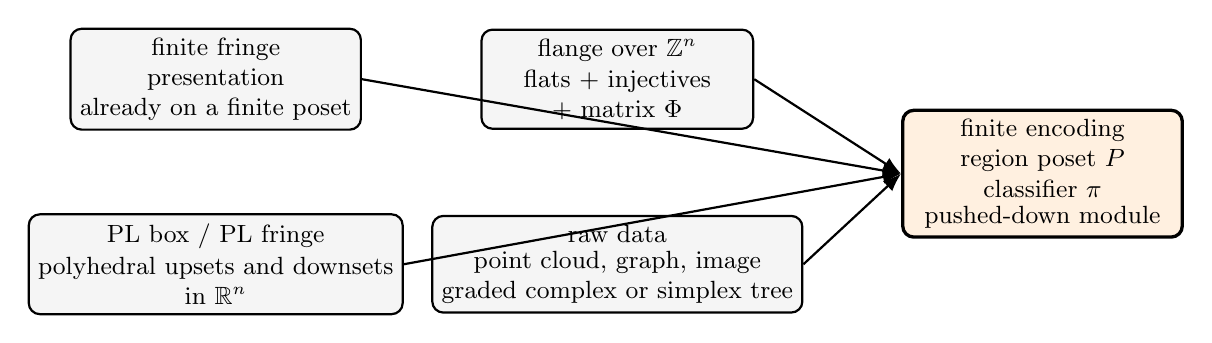
\begin{tikzpicture}[
  >=Latex,
  every node/.style={font=\small},
  src/.style={rounded corners, draw, thick, align=center, minimum width=3.45cm, minimum height=1.15cm, fill=gray!8},
  enc/.style={rounded corners, draw, very thick, align=center, minimum width=3.55cm, minimum height=1.2cm, fill=orange!12}
]
\node[src] (finite) at (-5.1,1.35) {\shortstack{finite fringe\\presentation\\already on a finite poset}};
\node[src] (flange) at (0,1.35) {\shortstack{flange over $\Z^n$\\flats + injectives\\+ matrix $\Phi$}};
\node[src] (pl) at (-5.1,-1.0) {\shortstack{PL box / PL fringe\\polyhedral upsets and downsets\\in $\R^n$}};
\node[src] (raw) at (0,-1.0) {\shortstack{raw data\\point cloud, graph, image\\graded complex or simplex tree}};
\node[enc] (enc) at (5.4,0.15) {\shortstack{finite encoding\\region poset $P$\\classifier $\pi$\\pushed-down module}};
\draw[->,thick] (finite.east) -- (enc.west);
\draw[->,thick] (flange.east) -- (enc.west);
\draw[->,thick] (pl.east) -- (enc.west);
\draw[->,thick] (raw.east) -- (enc.west);
\end{tikzpicture}

\medskip
\raggedright
The implementation keeps the front end heterogeneous, then forces all four inputs into one finite internal language.
\end{frame}

\begin{frame}{The universal idea: signatures and constant regions}
\small
For a presentation
\[
\varphi:\bigoplus_i \kk\{U_i\} \longrightarrow \bigoplus_j \kk\{D_j\},
\]
we classify each parameter value $q$ by the signature
\[
\sigma(q)=(y(q),z(q)),
\qquad
y_i(q)=1\iff q\in U_i,
\qquad
z_j(q)=1\iff q\notin D_j.
\]
Equal signatures mean the same active generators and relations, hence the same local presentation matrix.

\medskip
\centering
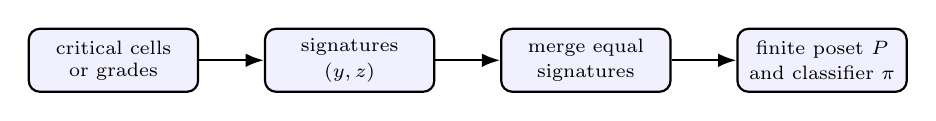
\begin{tikzpicture}[
  >=Latex,
  every node/.style={font=\scriptsize},
  box/.style={rounded corners, draw, thick, align=center, minimum width=2.15cm, minimum height=0.8cm, fill=blue!6}
]
\node[box] (cells) at (-4.5,0) {\shortstack{critical cells\\or grades}};
\node[box] (sig) at (-1.5,0) {\shortstack{signatures\\$(y,z)$}};
\node[box] (merge) at (1.5,0) {\shortstack{merge equal\\signatures}};
\node[box] (poset) at (4.5,0) {\shortstack{finite poset $P$\\and classifier $\pi$}};
\draw[->,thick] (cells) -- (sig);
\draw[->,thick] (sig) -- (merge);
\draw[->,thick] (merge) -- (poset);
\end{tikzpicture}

\medskip
\raggedright
This signature-first pattern is the common core of every backend.
\end{frame}

\begin{frame}{Encoding a flange over $\Z^n$}
\small
A flange input consists of flats, injectives, and a matrix $\Phi$.  The encoder uses the fact that membership can change only across finitely many coordinate thresholds.

\begin{itemize}
  \item extract critical coordinates on each axis;
  \item cut $\Z^n$ into slab cells;
  \item evaluate signatures on slab representatives;
  \item merge equal signatures into a finite signature poset;
  \item push the presentation down to a finite fringe module on $P$.
\end{itemize}

\raggedright
Implementation details that matter in practice: bit-packed signatures, reusable slab traversal, and common encoding for several flanges at once.

\end{frame}


\begin{frame}{Encoding a flange over $\Z^n$}
\centering
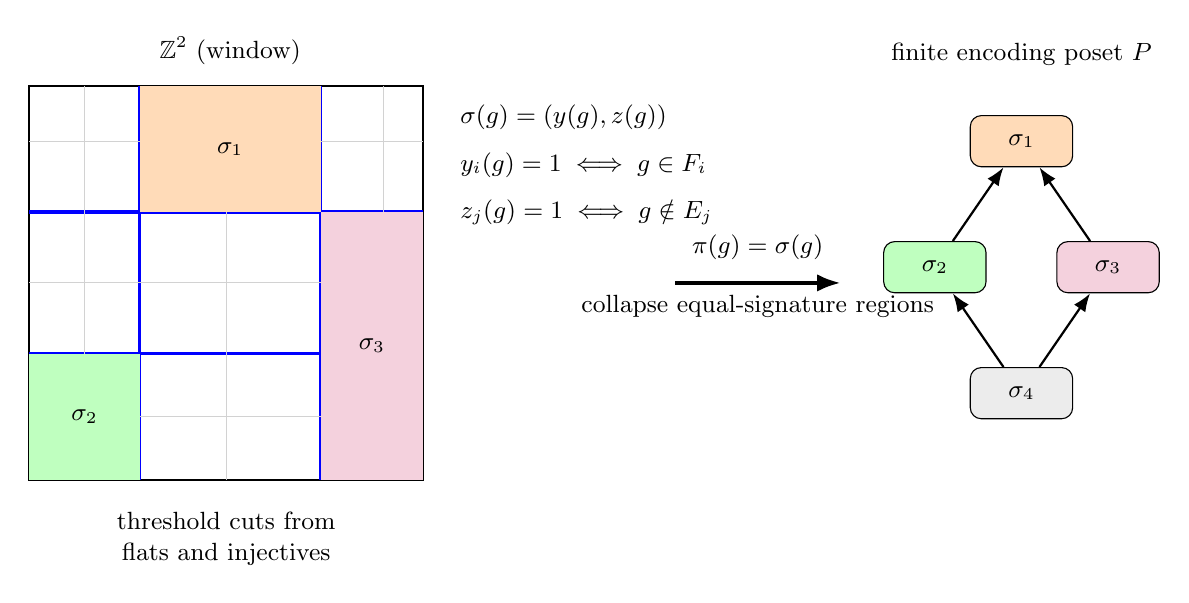
\begin{tikzpicture}[
	x=1cm,y=1cm,
	>=Latex,
	every node/.style={font=\small}
	]
	
	% --------------------------
	% Left panel: ambient Z^2 window
	% --------------------------
	\begin{scope}
		% outer box
		\draw[thick] (0,0) rectangle (5,5);
		
		% threshold cuts (non-uniform)
		\draw[blue, very thick] (1.4,0) -- (1.4,5);
		\draw[blue, very thick] (3.7,0) -- (3.7,5);
		\draw[blue, very thick] (0,1.6) -- (5,1.6);
		\draw[blue, very thick] (0,3.4) -- (5,3.4);
		
		% faint auxiliary grid to suggest lattice/slabs
		\draw[gray!35] (0.7,0) -- (0.7,5);
		\draw[gray!35] (2.5,0) -- (2.5,5);
		\draw[gray!35] (4.5,0) -- (4.5,5);
		\draw[gray!35] (0,0.8) -- (5,0.8);
		\draw[gray!35] (0,2.5) -- (5,2.5);
		\draw[gray!35] (0,4.3) -- (5,4.3);
		
		% highlighted regions
		\fill[green!25] (0,0) rectangle (1.4,1.6);
		\fill[orange!28] (1.4,3.4) rectangle (3.7,5);
		\fill[purple!18] (3.7,0) rectangle (5,3.4);
		
		% labels
		\node at (2.55,5.45) {$\mathbb{Z}^2$ (window)};
		\node[align=center] at (2.5,-0.75) {threshold cuts from\\flats and injectives};
		
		\node at (0.7,0.8) {$\sigma_2$};
		\node at (2.55,4.2) {$\sigma_1$};
		\node at (4.35,1.7) {$\sigma_3$};
		
		% annotation of what causes signatures
		\node[align=left, anchor=west] at (5.35,4.6) {$\sigma(g)=(y(g),z(g))$};
		\node[align=left, anchor=west] at (5.35,4.0) {$y_i(g)=1 \iff g\in F_i$};
		\node[align=left, anchor=west] at (5.35,3.4) {$z_j(g)=1 \iff g\notin E_j$};
	\end{scope}
	
	% --------------------------
	% Arrow and classifier label
	% --------------------------
	\draw[->, very thick] (8.2,2.5) -- (10.3,2.5);
	\node at (9.25,2.95) {$\pi(g)=\sigma(g)$};
	\node at (9.25,2.2) {collapse equal-signature regions};
	
	% --------------------------
	% Right panel: finite poset P
	% --------------------------
	\begin{scope}[shift={(11.2,0.2)}]
		\node at (1.4,5.2) {finite encoding poset $P$};
		
		% nodes
		\node[draw, rounded corners, fill=orange!28, minimum width=1.3cm, minimum height=0.65cm] (s1) at (1.4,4.1) {$\sigma_1$};
		\node[draw, rounded corners, fill=green!25, minimum width=1.3cm, minimum height=0.65cm] (s2) at (0.3,2.5) {$\sigma_2$};
		\node[draw, rounded corners, fill=purple!18, minimum width=1.3cm, minimum height=0.65cm] (s3) at (2.5,2.5) {$\sigma_3$};
		\node[draw, rounded corners, fill=gray!15, minimum width=1.3cm, minimum height=0.65cm] (s4) at (1.4,0.9) {$\sigma_4$};
		
		% order relations
		\draw[->, thick] (s2) -- (s1);
		\draw[->, thick] (s3) -- (s1);
		\draw[->, thick] (s4) -- (s2);
		\draw[->, thick] (s4) -- (s3);
	\end{scope}
	
\end{tikzpicture}

\end{frame}

\begin{frame}{Encoding flanges over $\mathbb{Z}^n$: slab cells}
	\centering
	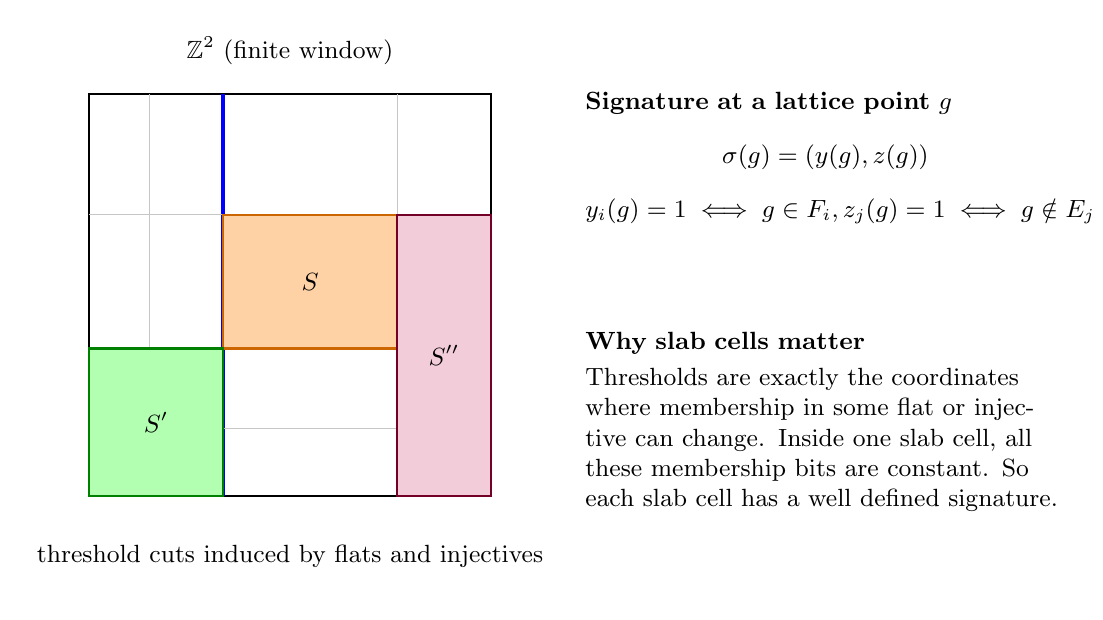
\begin{tikzpicture}[
		x=0.85cm,y=0.85cm,
		>=Latex,
		every node/.style={font=\small}
		]
		
		% =========================
		% Left: threshold window in Z^2
		% =========================
		\begin{scope}
			% outer box
			\draw[thick] (0,0) rectangle (6,6);
			
			% slab / threshold cuts
			\draw[gray!45] (0.9,0) -- (0.9,6);
			\draw[blue, very thick] (2.0,0) -- (2.0,6);
			\draw[gray!45] (4.6,0) -- (4.6,6);
			
			\draw[gray!45] (0,1.0) -- (6,1.0);
			\draw[blue, very thick] (0,2.2) -- (6,2.2);
			\draw[gray!45] (0,4.2) -- (6,4.2);
			
			% highlighted slab cells
			\fill[orange!35] (2.0,2.2) rectangle (4.6,4.2);
			\draw[thick, orange!80!black] (2.0,2.2) rectangle (4.6,4.2);
			\node at (3.3,3.2) {$S$};
			
			\fill[green!30] (0,0) rectangle (2.0,2.2);
			\draw[thick, green!50!black] (0,0) rectangle (2.0,2.2);
			\node at (1.0,1.1) {$S'$};
			
			\fill[purple!20] (4.6,0) rectangle (6.0,4.2);
			\draw[thick, purple!60!black] (4.6,0) rectangle (6.0,4.2);
			\node at (5.3,2.1) {$S''$};
			
			% title and caption
			\node at (3,6.65) {$\mathbb{Z}^2$ (finite window)};
			\node[align=center] at (3,-0.9)
			{threshold cuts induced by flats and injectives};
		\end{scope}
		
		% =========================
		% Middle: signature definitions
		% =========================
		\begin{scope}[shift={(11,0.7)}]
			\node[align=left, text width=6.1cm] at (0,4.35) {
				\textbf{Signature at a lattice point $g$}
				\[
				\sigma(g)=(y(g),z(g))
				\]
				\[
				y_i(g)=1 \iff g\in F_i,
				z_j(g)=1 \iff g\notin E_j
				\]
			};
			
			\node[align=left, text width=6.1cm] at (0,0.4) {
				\textbf{Why slab cells matter}\\[0.2em]
				Thresholds are exactly the coordinates where
				membership in some flat or injective can change.
				Inside one slab cell, all these membership bits are constant.
				So each slab cell has a well defined signature.
			};
			
			\node[align=left, text width=6.1cm] at (0,-2) {
				
			};
		\end{scope}
	\end{tikzpicture}
\end{frame}

\begin{frame}{Encoding flanges over $\mathbb{Z}^n$: quotient by signature}
	\centering
	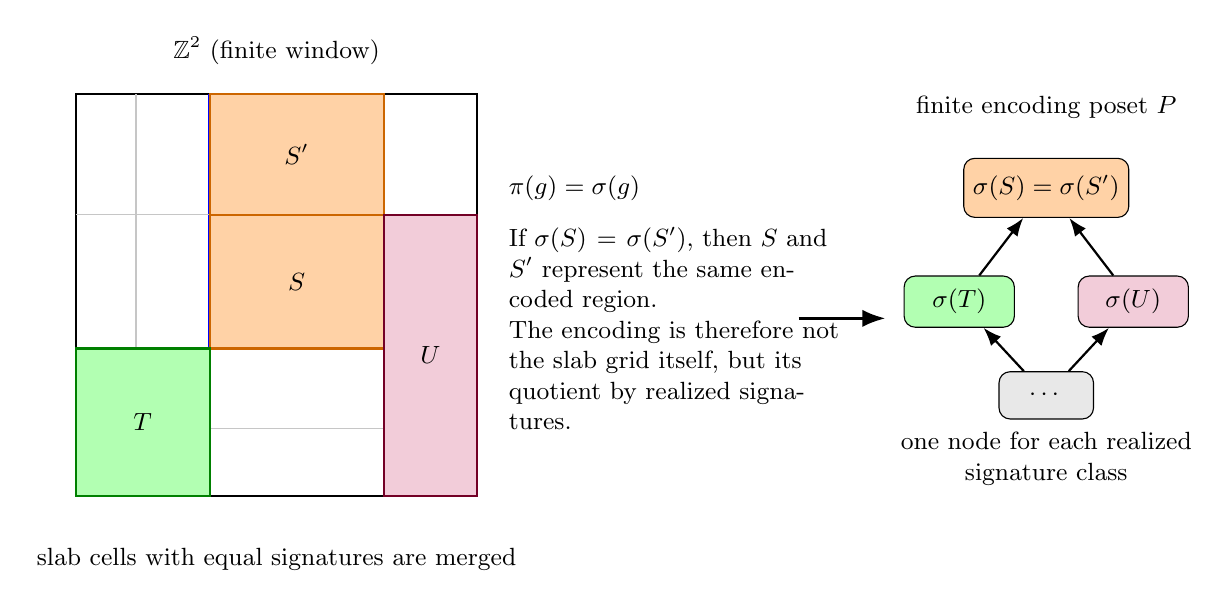
\begin{tikzpicture}[
		x=0.85cm,y=0.85cm,
		>=Latex,
		every node/.style={font=\small}
		]
		
		% =========================
		% Left: slab cells, with equal-signature regions
		% =========================
		\begin{scope}
			% outer box
			\draw[thick] (0,0) rectangle (6,6);
			
			% slab / threshold cuts
			\draw[gray!45] (0.9,0) -- (0.9,6);
			\draw[blue, very thick] (2.0,0) -- (2.0,6);
			\draw[gray!45] (4.6,0) -- (4.6,6);
			
			\draw[gray!45] (0,1.0) -- (6,1.0);
			\draw[blue, very thick] (0,2.2) -- (6,2.2);
			\draw[gray!45] (0,4.2) -- (6,4.2);
			
			% equal-signature slab cells
			\fill[orange!35] (2.0,2.2) rectangle (4.6,4.2);
			\draw[thick, orange!80!black] (2.0,2.2) rectangle (4.6,4.2);
			\node at (3.3,3.2) {$S$};
			
			\fill[orange!35] (2.0,4.2) rectangle (4.6,6.0);
			\draw[thick, orange!80!black] (2.0,4.2) rectangle (4.6,6.0);
			\node at (3.3,5.1) {$S'$};
			
			\fill[green!30] (0,0) rectangle (2.0,2.2);
			\draw[thick, green!50!black] (0,0) rectangle (2.0,2.2);
			\node at (1.0,1.1) {$T$};
			
			\fill[purple!20] (4.6,0) rectangle (6.0,4.2);
			\draw[thick, purple!60!black] (4.6,0) rectangle (6.0,4.2);
			\node at (5.3,2.1) {$U$};
			
			% title and caption
			\node at (3,6.65) {$\mathbb{Z}^2$ (finite window)};
			\node[align=center] at (3,-0.95)
			{slab cells with equal signatures are merged};
		\end{scope}
		
		% =========================
		% Middle: quotient statement
		% =========================
		\begin{scope}[shift={(9,1.0)}]
			\node[align=left, text width=4.3cm] at (0,3.6) {
				$\pi(g)=\sigma(g)$
			};
			
			\node[align=left, text width=4.3cm] at (0,1.5) {
				If $\sigma(S)=\sigma(S')$, then \(S\) and \(S'\) represent the same encoded region. \\
				The encoding is therefore not the slab grid itself, but its quotient by realized signatures.
			};
			
			\node[align=left, text width=4.3cm] at (0,0.5) {
				
			};
		\end{scope}
		
		% arrow
		\draw[->, very thick] (10.8,2.65) -- (12.1,2.65);
		
		% =========================
		% Right: finite poset P
		% =========================
		\begin{scope}[shift={(12.8,0.8)}]
			\node at (1.7,5.0) {finite encoding poset $P$};
			
			\node[draw, rounded corners, fill=orange!35, minimum width=2.0cm, minimum height=0.75cm] (s1) at (1.7,3.8) {$\sigma(S)=\sigma(S')$};
			\node[draw, rounded corners, fill=green!30, minimum width=1.4cm, minimum height=0.65cm] (s2) at (0.4,2.1) {$\sigma(T)$};
			\node[draw, rounded corners, fill=purple!20, minimum width=1.4cm, minimum height=0.65cm] (s3) at (3.0,2.1) {$\sigma(U)$};
			\node[draw, rounded corners, fill=gray!18, minimum width=1.2cm, minimum height=0.6cm] (s4) at (1.7,0.7) {$\cdots$};
			
			\draw[->, thick] (s2) -- (s1);
			\draw[->, thick] (s3) -- (s1);
			\draw[->, thick] (s4) -- (s2);
			\draw[->, thick] (s4) -- (s3);
			
			\node[align=center] at (1.7,-0.25)
			{one node for each realized\\signature class};
		\end{scope}
		
	\end{tikzpicture}
\end{frame}

\begin{frame}{Encoding PL box presentations}
\small
For axis-aligned boxes in $\R^n$, the geometry is simpler and the traversal can be specialized.

\begin{itemize}
  \item collect all lower and upper coordinate thresholds;
  \item build the rectangular cell grid they induce;
  \item traverse cells in odometer order;
  \item update signatures incrementally when a threshold is crossed;
  \item build a direct cell-to-region lookup table.
\end{itemize}

\medskip
\raggedright
This backend is faster because it avoids generic polyhedral feasibility and uses mixed-radix indexing for point location.
\end{frame}

\begin{frame}{Encoding PL box presentations: threshold cells}
	\centering
	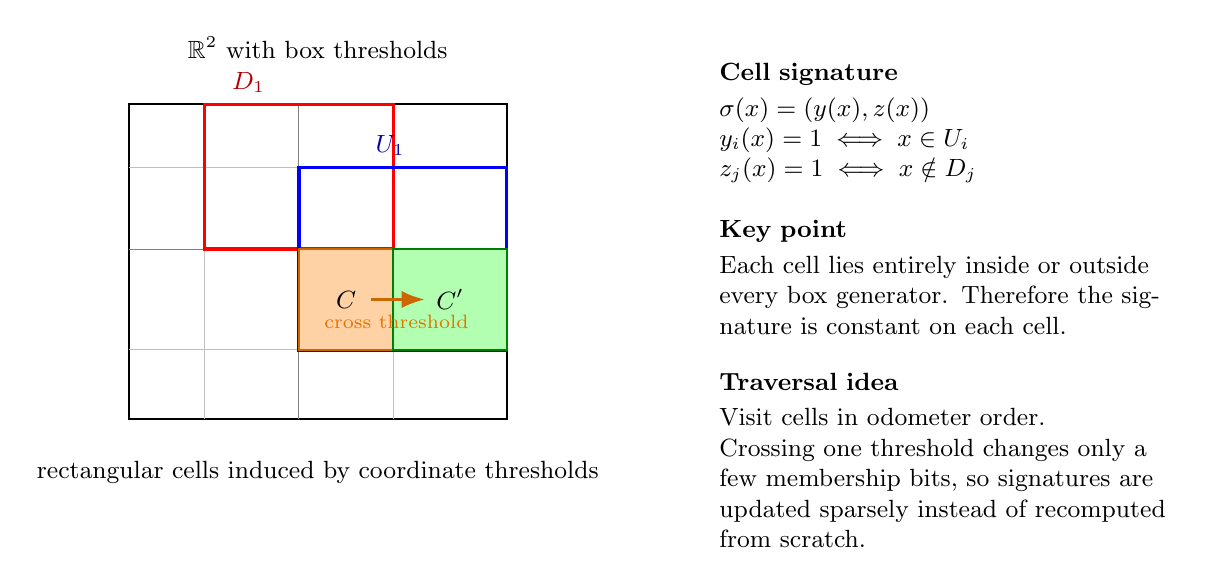
\begin{tikzpicture}[
		x=0.8cm,y=0.8cm,
		>=Latex,
		every node/.style={font=\small}
		]
		
		% =========================
		% Left: threshold grid
		% =========================
		\begin{scope}
			% outer box
			\draw[thick] (0,0) rectangle (6,5);
			
			% threshold lines
			\draw[gray!50] (1.2,0) -- (1.2,5);
			\draw[gray] (2.7,0) -- (2.7,5);
			\draw[gray!50] (4.2,0) -- (4.2,5);
			
			\draw[gray!50] (0,1.1) -- (6,1.1);
			\draw[gray] (0,2.7) -- (6,2.7);
			\draw[gray!50] (0,4.0) -- (6,4.0);
			
			% box supports
			\draw[red, very thick] (1.2,2.7) rectangle (4.2,5.0);
			\node[red!70!black] at (1.9,5.35) {$D_1$};
			
			\draw[blue, very thick] (2.7,1.1) rectangle (6,4.0);
			\node[blue!70!black] at (4.15,4.35) {$U_1$};
			
			% current and next cells
			\fill[orange!35] (2.7,1.1) rectangle (4.2,2.7);
			\draw[thick, orange!80!black] (2.7,1.1) rectangle (4.2,2.7);
			\node at (3.45,1.9) {$C$};
			
			\fill[green!30] (4.2,1.1) rectangle (6.0,2.7);
			\draw[thick, green!50!black] (4.2,1.1) rectangle (6.0,2.7);
			\node at (5.1,1.9) {$C'$};
			
			% traversal arrow
			\draw[->, very thick, orange!80!black] (3.85,1.9) -- (4.7,1.9);
			\node[orange!90!black] at (4.25,1.55) {\scriptsize cross threshold};
			
			% title and caption
			\node at (3,5.9) {$\mathbb{R}^2$ with box thresholds};
			\node[align=center] at (3,-0.85)
			{rectangular cells induced by coordinate thresholds};
		\end{scope}
		
		% =========================
		% Right: signature explanation
		% =========================
		\begin{scope}[shift={(13,0.5)}]
			\node[align=left, text width=5.8cm] at (0,4.2) {
				\textbf{Cell signature}\\[0.2em]
				$\sigma(x)=(y(x),z(x))$\\
				$y_i(x)=1 \iff x\in U_i$\\
				$z_j(x)=1 \iff x\notin D_j$
			};
			
			\node[align=left, text width=5.8cm] at (0,1.75) {
				\textbf{Key point}\\[0.2em]
				Each cell lies entirely inside or outside\\
				every box generator. Therefore the signature
				is constant on each cell.
			};
			
			\node[align=left, text width=5.8cm] at (0,-1.15) {
				\textbf{Traversal idea}\\[0.2em]
				Visit cells in odometer order.\\
				Crossing one threshold changes only a few
				membership bits, so signatures are updated
				sparsely instead of recomputed from scratch.
			};
		\end{scope}
		
	\end{tikzpicture}
\end{frame}

\begin{frame}{Encoding PL box presentations: quotient by signature}
	\centering
	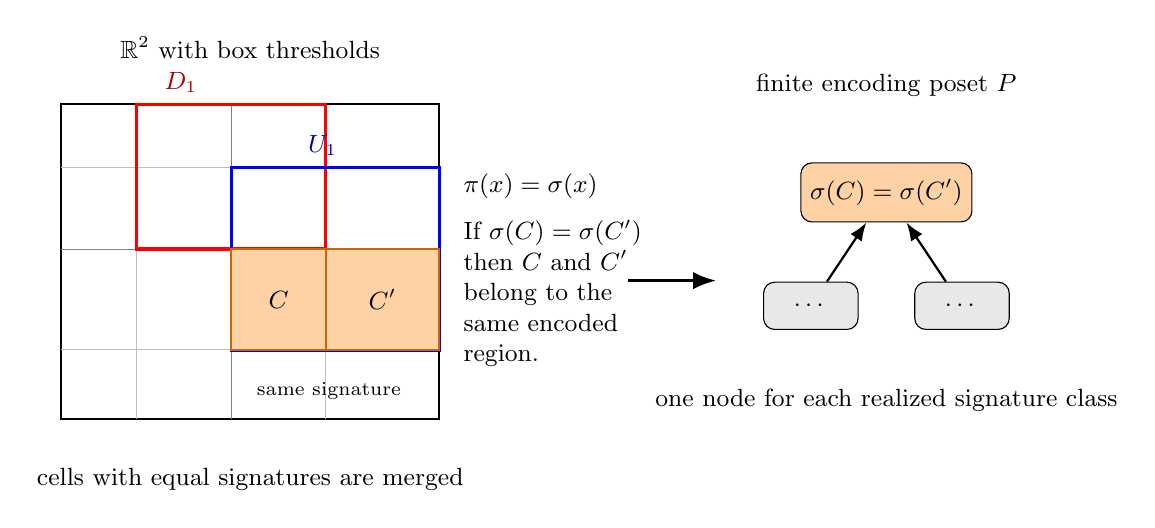
\begin{tikzpicture}[
		x=0.8cm,y=0.8cm,
		>=Latex,
		every node/.style={font=\small}
		]
		
		% =========================
		% Left: threshold grid with same-signature cells
		% =========================
		\begin{scope}
			% outer box
			\draw[thick] (0,0) rectangle (6,5);
			
			% threshold lines
			\draw[gray!50] (1.2,0) -- (1.2,5);
			\draw[gray] (2.7,0) -- (2.7,5);
			\draw[gray!50] (4.2,0) -- (4.2,5);
			
			\draw[gray!50] (0,1.1) -- (6,1.1);
			\draw[gray] (0,2.7) -- (6,2.7);
			\draw[gray!50] (0,4.0) -- (6,4.0);
			
			% box supports
			\draw[red, very thick] (1.2,2.7) rectangle (4.2,5.0);
			\node[red!70!black] at (1.9,5.35) {$D_1$};
			
			\draw[blue, very thick] (2.7,1.1) rectangle (6,4.0);
			\node[blue!70!black] at (4.15,4.35) {$U_1$};
			
			% equal-signature cells
			\fill[orange!35] (2.7,1.1) rectangle (4.2,2.7);
			\draw[thick, orange!80!black] (2.7,1.1) rectangle (4.2,2.7);
			
			\fill[orange!35] (4.2,1.1) rectangle (6.0,2.7);
			\draw[thick, orange!80!black] (4.2,1.1) rectangle (6.0,2.7);
			
			\node at (3.45,1.9) {$C$};
			\node at (5.1,1.9) {$C'$};
			
			% brace-like annotation
			\node[align=center] at (4.25,0.45) {\scriptsize same signature};
			
			% title and caption
			\node at (3,5.9) {$\mathbb{R}^2$ with box thresholds};
			\node[align=center] at (3,-0.95)
			{cells with equal signatures are merged};
		\end{scope}
		
		% =========================
		% Middle: classifier statement
		% =========================
		\begin{scope}[shift={(8.7,0)}]
			\node[align=left, text width=3.7cm] at (0,3.7) {
				$\pi(x)=\sigma(x)$
			};
			\node[align=left, text width=3.7cm] at (0,2.0) {
				If $\sigma(C)=\sigma(C')$ \\
				then \(C\) and \(C'\) \\
				belong to the \\
				same encoded \\
				region.
			};
		\end{scope}
		
		% arrow
		\draw[->, very thick] (9.0,2.2) -- (10.4,2.2);
		
		% =========================
		% Right: finite poset
		% =========================
		\begin{scope}[shift={(11.5,0.5)}]
			\node at (1.6,4.8) {finite encoding poset $P$};
			
			\node[draw, rounded corners, fill=orange!35, minimum width=2.0cm, minimum height=0.75cm] (s1) at (1.6,3.1) {$\sigma(C)=\sigma(C')$};
			\node[draw, rounded corners, fill=gray!18, minimum width=1.2cm, minimum height=0.6cm] (s2) at (0.4,1.3) {$\cdots$};
			\node[draw, rounded corners, fill=gray!18, minimum width=1.2cm, minimum height=0.6cm] (s3) at (2.8,1.3) {$\cdots$};
			
			\draw[->, thick] (s2) -- (s1);
			\draw[->, thick] (s3) -- (s1);
			
			\node[align=center] at (1.6,-0.2)
			{one node for each realized signature class};
		\end{scope}
		
	\end{tikzpicture}
\end{frame}

\begin{frame}{Encoding general PL fringes}
\small
For genuine polyhedral upsets and downsets, the backend is signature-first rather than arrangement-first.

\begin{itemize}
  \item store each convex piece by exact halfspaces over $\Q$;
  \item avoid building the full arrangement;
  \item ``inside a union'' is handled by choosing a piece;
  \item ``outside a union'' is handled by choosing a facet inequality to violate;
  \item solve exact feasibility only for candidate signatures;
  \item cache witness points and float surrogates for later point location.
\end{itemize}

\centering
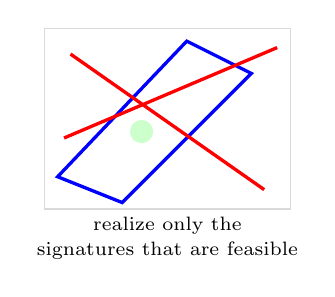
\begin{tikzpicture}[scale=0.82, every node/.style={font=\scriptsize}]
  \draw[gray!30,thin] (0,0) rectangle (3.8,2.8);
  \draw[very thick,blue] (0.2,0.5) -- (2.2,2.6) -- (3.2,2.1) -- (1.2,0.1) -- cycle;
  \draw[very thick,red] (0.4,2.4) -- (3.4,0.3);
  \draw[very thick,red] (0.3,1.1) -- (3.6,2.5);
  \fill[green!20] (1.5,1.2) circle (0.18);
  \node[align=center] at (1.9,-0.45) {\shortstack{realize only the\\signatures that are feasible}};
\end{tikzpicture}

\medskip
\raggedright
This is what makes richer polyhedral geometry tractable while keeping the encoded result exact.
\end{frame}

\begin{frame}{From raw data to an encoded module}
\small
Raw data passes through a finite graded object before encoding.

\medskip
\centering
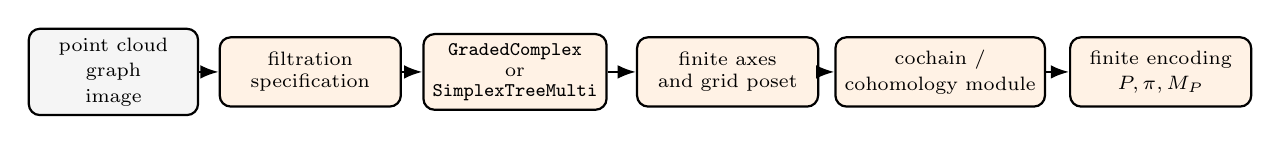
\begin{tikzpicture}[
  >=Latex,
  every node/.style={font=\scriptsize},
  box/.style={rounded corners, draw, thick, align=center, minimum width=2.15cm, minimum height=0.8cm, fill=gray!8},
  stage/.style={rounded corners, draw, thick, align=center, minimum width=2.3cm, minimum height=0.88cm, fill=orange!10}
]
\node[box] (raw) at (-5.7,0) {\shortstack{point cloud\\graph\\image}};
\node[stage] (filt) at (-3.2,0) {\shortstack{filtration\\specification}};
\node[stage] (gc) at (-0.6,0) {\shortstack{\texttt{GradedComplex}\\or\\\texttt{SimplexTreeMulti}}};
\node[stage] (axes) at (2.1,0) {\shortstack{finite axes\\and grid poset}};
\node[stage] (coh) at (4.8,0) {\shortstack{cochain /\\cohomology module}};
\node[stage] (enc) at (7.6,0) {\shortstack{finite encoding\\$P,\pi,M_P$}};
\draw[->,thick] (raw) -- (filt);
\draw[->,thick] (filt) -- (gc);
\draw[->,thick] (gc) -- (axes);
\draw[->,thick] (axes) -- (coh);
\draw[->,thick] (coh) -- (enc);
\end{tikzpicture}

\medskip
\raggedright
The key point is that data-derived modules and presentation-derived modules meet at the same endpoint: a finite encoded module on a finite poset.
\end{frame}

\begin{frame}{What the classifier stores, and why it matters}
\small
The classifier is not just a formal map $\pi:Q\to P$.  It is a compiled object used repeatedly by later routines.

\medskip
\begin{tabularx}{\textwidth}{>{\raggedright\arraybackslash}p{3.7cm}X}
\toprule
Stored information & Why it matters \\
\midrule
region representatives, axes, cell lookup & fast point location and batched queries \\
realized signatures and finite poset structure & exact pushed-down module and naturality of maps \\
region geometry: weights, bounding boxes, adjacency & weighted invariants, support summaries, visualization \\
cache fingerprints and compiled metadata & reuse across repeated computations and common encodings \\
\bottomrule
\end{tabularx}

\medskip
This is why the output is an \texttt{EncodingResult} rather than a bare finite poset.
\end{frame}

\begin{frame}{Takeaways}
\small
\begin{enumerate}
  \item Four very different front ends are accepted: finite fringes, flanges, PL presentations, and raw filtered data.
  \item All of them are turned into the same internal object: a finite poset, a finite module on that poset, and a compiled classifier map.
  \item The universal mechanism is signature-based: identify constant regions, realize only the signatures that occur, then push the module down.
  \item The backend changes with the geometry:
  \begin{itemize}
    \item flange: slab cells in $\Z^n$;
    \item PL box: rectangular traversal with sparse updates;
    \item general PL: exact feasibility on candidate signatures;
    \item raw data: graded complexes or simplex trees, then cohomology on a finite grid.
  \end{itemize}
  \item Once the encoding exists, all later algebra and invariants work from the same finite object.
\end{enumerate}
\end{frame}

\begin{frame}{Selected references}
\footnotesize
\begin{itemize}
  \item E. Miller, \emph{Homological algebra of modules over posets}, 2020.
  \item M. Lesnick, \emph{The theory of the interleaving distance on multidimensional persistence modules}, 2015.
  \item M. Lesnick and M. Wright, \emph{Interactive visualization of 2-D persistence modules}, 2015.
  \item M. Kerber, M. Lesnick, and S. Oudot, \emph{Exact computation of the matching distance on 2-parameter persistence modules}, 2020.
  \item M. Carriere and A. Blumberg, \emph{Multiparameter persistence image for topological machine learning}, 2020.
\end{itemize}
\end{frame}

\end{document}
